\section{DnsName}\label{sec:dnsname}

\begin{figure}
\begin{center}
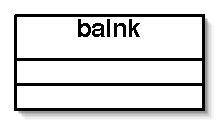
\includegraphics[width=0.4\textwidth]{figs/blank}
\end{center}
\caption{}
\label{fig:dnsname}
\end{figure}

This section describes the DnsName component, which is described by Figure~\ref{fig:dnsname}.  

This class implements the semantics of a DNS name. Due to the use of DNS-style compression, handling of DNS names is non-trivial.

\subsection{Methods}

{\bf Public Methods}
\begin{itemize}
\item from\_wire(): A factory method which parses a name from the wire and returns an object of the DnsName class on successful parse.
\item to\_wire(): Takes a name length and an optional pointer and converts the name into a compressed wire representation.
\end{itemize}

{\bf Private Methods}
\begin{itemize}
\item empty\_list(): Frees memory associated with the object.
\item read\_name(): Reads a name from a packet, handling compression as needed.
\end{itemize}

\subsection{Member Variables}
\begin{itemize}
\item m\_parts: List of the period-delimited parts of the DNS name.
\item m\_length: Length of the uncompressed name.
\end{itemize}
